% !TeX root = RJwrapper.tex
\title{Fitting Explainable Boosting Machines in R with the ebm Package}
\author{by Brandon M. Greenwell}

\maketitle

\abstract{%
An abstract of less than 150 words.
}

\subsection{Introduction}\label{introduction}

Generalized linear models (GLMs) \citep{nelder-1972-glm} have been a
bedrock of statistical modeling for over fifty years. GLMs extend the
classic linear model to accommodate non-Gaussian response distributions,
as well as some degree of non-linearity in the model structure. In
particular, GLMs have three components:

\begin{enumerate}
\def\labelenumi{\arabic{enumi}.}
\item
  A random component, which specifies a distribution for the response
  \(Y\) conditional on a set of predictors \(\boldsymbol{x}\). In a
  traditional linear model, for instance, \(Y|\boldsymbol{x}\) is often
  assumed to have a Gaussian (or normal) distribution with constant
  variance \(\sigma^2\).
\item
  A systematic component, which specifies a linear combination of the
  regression coefficients and the predictors and is often called the
  \emph{linear predictor}:
  \(\eta = \beta_0 + \beta_1x_1 + \cdots + \beta_px_p = \boldsymbol{x}^\top\boldsymbol{\beta}\).
  (Note that linear here refers to the fact that \(\eta\) is linear in
  the regression coefficients \(\boldsymbol{\beta}\).)
\item
  A link function, which specifies how the linear predictor (systematic
  component) is linked to the conditional mean response
  \(\mathrm{E}\left(Y|\boldsymbol{x}\right)\) (random component). In
  logistic regression, for instance, this is the logit function.
\end{enumerate}

In essence, GLMs have the following basic form: \begin{equation*}
  g\left(E\left[Y|\boldsymbol{x}\right]\right) = \beta_0 + \sum_{j=1}^p \beta_jx_j,
\end{equation*} where \(Y \sim\) some exponential family distribution,
\(g\) is the link function (e.g., typically the identity function for
linear models, the logit for logistic regression, or the log link for
Poisson regression), and
\(\boldsymbol{\beta} = \left(\beta_0, \beta_1, \dots, \beta_p\right)^\top\)
are fixed but unknown regression coefficients to be estimated from the
data (typically, via some form of maximum likelihood estimation). The
definitive reference for GLMs has always been the monograph by
\citet{mccullagh-1989-glm}.

Generalized additive models (GAMs) \citep{hastie-1990-gam} extend GLMs
by replacing the systematic component of @ref(eq:glm) with a sum of
nonlinear smooth functions to get \begin{equation}
  g\left(E\left[Y|\boldsymbol{x}\right]\right) = \beta_0 + \sum_{j=1}^p f_j\left(x_j\right),
  \label{eqn:gam}
\end{equation} The functions \(f_j\) are general enough that they can
absorb the intercept (hence, sometimes we may omit the bias term
\(\beta_0\) in \eqref{eqn:gam}). Model \eqref{eqn:gam} is quite flexible
in how the response depends on the predictors. Further, GAMs maintain
explainability since the model's output can be understood by simply
plotting the individual term contributions (sometimes called shape
functions) \(f_j\left(x_j\right)\). GAMs can also include interactions
effects. For example, a pairwise interaction effect between \(x_i\) and
\(x_j\) can be accommodated by including a bivariate term of the form
\(f\left(x_i, x_j\right)\). The terms in a GAM can be represented by a
variety of functions. Traditionally, the terms in a GAM are represented
using some form of smoothing splines. For a thorough overview of GAMs,
see \citet{wood-2017-gam}.

\citet{lou-2013-ga2m} introduced generalized additive models plus
interactions (GA\textsuperscript{2}Ms) which automatically search for
and include important pairwise interaction terms using an algorith
called FAST\footnote{As far as I can tell, FAST is not an acronym for
  anything in particular.}. The resulting model consists of univariate
terms and a small number of pairwise interaction terms. Since
GA\textsuperscript{2}Ms are low-dimensional, they can still be
visualized and interpreted by users while potentially being more
accurate. A GA\textsuperscript{2}M has the general form \begin{equation}
  g\left(E\left[Y|\boldsymbol{x}\right]\right) = \sum f_i\left(x_i\right) + \sum f_{ij}\left(x_i, x_j\right).
  \label{eqn:ga2m}
\end{equation} Here we've simply abosrbed the bias term (or intercept)
into the shape functions \(f_i\). In contrast to tradition GAMs
\eqref{eqn:gam}, the shape functions in \eqref{eqn:ga2m} are not
necessarily smooth. In particular, modern GA\textsuperscript{2}Ms often
rely on tree-based methods and gradient boosting
\citep{greenwell-2022-tree}, which tend to produce more rigid step
functions.

\section{Explainable boosting
machines}\label{explainable-boosting-machines}

Explainable boosting machines \citep{nori-2019-interpret}, or EBMs for
short, are a modern class of GA\textsuperscript{2}Ms, that can offer
both competitive accuracy and explicit transparency and explainability,
which are often considered to be two opposing goals of a machine
learning (ML) model. For example, full-complexity models, like random
forests \citep{breiman-2001-rf}, tend to be highly competitive in terms
of accuracy, but are readily less transparent and explainable (due in
part to the high-order interaction effects often captured by such
black-box models). Essentially, with EBMs, it's possible to ``have your
cake and eat it too.'\,'

In short, EBM models have the general form

\begin{equation}
g\left(E\left[y\right]\right) = \theta_0 + \sum f_i\left(x_i\right) + \sum f_{ij}\left(x_i, x_j\right),
  \label{eqn:ebm}
\end{equation}

Where blah, blah, blah @ref(eq:ga2m)

where

\begin{itemize}
\item
  \(g\) is a \emph{link function} that allows the model to handle
  various response types (e.g., the \emph{logit} link for logistic
  regression or the identify function for ordinary regression with
  continuous outcomes);
\item
  \(\theta_0\) is a constant intercept (or bias term);
\item
  \(f_i\) is the \emph{term contribution} (or \emph{shape function}) for
  predictor \(x_i\) (i.e., it captures the main effect of \(x_i\));
\item
  \(f_{ij}\) is the term contribution for the pair of predictors \(x_i\)
  and \(x_j\) (i.e., it captures the joint effect, or pairwise
  interaction effect of \(x_i\) and \(x_j\)).
\end{itemize}

Similar to \emph{generalized additive models plus interactions} (Lou et
al.~2013), or GA\textsuperscript{2}Ms for short, the pairwise
interaction terms are determined automatically using the FAST algorithm
described in Lou et al.~(2013). In short, FAST is a novel,
computationally efficient method for ranking all possible pairs of
feature candidates for inclusion into the model (by default, the top 10
pairwise interactions are used). The primary difference between EBMs and
GA\textsuperscript{2}Ms is in how the shape functions are estimated. In
particular, EBMs use \emph{cyclic gradient boosting} (Nori et al.~2019;
Wick, Kerzel, and Feindt 2020) to estimate the shape functions for each
feature (and selected pairs of interactions) in a round-robin fashion
using a low learning rate to help ensure that the order in which the
feature effects are estimated does not matter. Estimating each feature
one-at-a-time in a round-robin fashion also helps mitigate potential
issues with \emph{collinearity} between predictors (Nori et al.~2019;
Wick, Kerzel, and Feindt 2020).

TODO: Move the following sections to later and modify. Also, talk about
model editing and how EBMs are editable. Maybe a GAM-CHANGER example if
there's room?!

However, in contrast to the more common gradient boosting machine (J. H.
Friedman 2001, 2002), or GBM for short, which can ignore irrelevant
inputs, EBMs include at least one term in the model for each feature:
one main effect (\(f_i\)) for each predictor, and a term for each
selected pairwise interaction effect. This is due to the cyclic nature
of the underlying boosting framework. For example, an EBM applied to a
training set with \(p = 300\) features will result in a model with at
least 300 terms.

While EBMs are considered \emph{glass-box} models, an EBM with, say,
hundreds or thousands of terms, starts to become much less transparent
and explainable. Moreover, the larger the fitted model (i.e., the more
terms there are), then the more time it will take the EBM to make
predictions, making larger models less fit for deployment and
production.

To this end, we also propose in Section XYZ a way to introduce sparsity
into a fitted EBM by rescaling the individual terms (i.e., the \(f_i\)
and \(f_{ij}\)) via regression coefficients estimated from a method
called the LASSO (Tibshirani 1996). Consequently, by nature of the
\(L_1\) regularization enforced by the LASSO, many of these coefficients
can be estimated to be zero, resulting in a reduced EBM with far fewer
terms (and hopefully, comparable accuracy)!

\subsection{Software}\label{software}

EBMs are implemented as part of the \textbf{InterpretML} framework
\citep{nori-2019-interpret}, which includes both a Python and R
interface called \textbf{interpret}. While the Python implementation is
fully functional and rich with features (e.g., interactive graphics),
the R version \citep{R-interpret} currently lags behind. For instance,
the R interface only supports classification settings and limited
options (e.g., monotonic constraints are not currently supported).

Further, the plotting functionality of the R \pkg{interpret} package
only supports visualizing a single feature using static plots (i.e., no
interactive visualizations, no visualizations for pairwise interactions,
feature importance plots, or support for visualizing local
explanations). Because of these serious drawbacks, we've developed the
\CRANpkg{ebm} package, which is a full-featured R interface to the
Python \pkg{interpret} library powered by \CRANpkg{reticulate}
\citep{R-reticulate}.

In the next section, we'll discuss the \pkg{ebm} package in detail and
provide several examples that cannot be replicated through use of the
official \pkg{interpret} package in R.

\section{\texorpdfstring{The \pkg{ebm}
package}{The  package}}\label{the-package}

The \pkg{ebm} package is an R wrapper around the explainable boosting
functionality of the \pkg{interpret} module in Python, powered by
\CRANpkg{reticulate}. The main features of this package, especially when
compared to the R package \pkg{interpret}, include:

\begin{itemize}
\tightlist
\item
  Support for all the objective (i.e., loss) function provided by the
  Python modeule (e.g., Poisson devaince for modeling counts).
\item
  Static and interactive graphics for explaining the model.
\item
  Global and local explanations for a fitted model.
\item
  Convenient generic function like \texttt{print()}, \texttt{plot()},
  and \texttt{predict()}.
\item
  Support for loading in EBM models fit via the corresponding Python
  module.
\end{itemize}

\subsection{Predicting and explaining policy ownership (the CoIL 2000
challenge)}\label{predicting-and-explaining-policy-ownership-the-coil-2000-challenge}

In this section, we briefly describe a binary classification example
using data from the CoIL 2000 Challenge \citep{putten-2004-coil}. The
data set, which we'll obtain from the R package \CRANpkg{kernlab}
\citep{R-kernlab}, consists of 9822 customer records containing 86
variables, including product usage data and socio-demographic data
derived from zip area codes. The goal of the challenge was to be able to
answer the following question: ``Can you predict who would be interested
in buying a caravan insurance policy and give an explanation of why?'\,'
Hence, being able to explain your model's predictions was key to being
successful in this challenge.

To start, we'll load in the data and split into train/test sets using
the same partitioning as the original competition (see
\texttt{?kernlab::ticdata} for variable descriptions and further
details):

\begin{Schunk}
\begin{Sinput}
data("ticdata", package = "kernlab")
ticdata$CARAVAN <- ifelse(ticdata$CARAVAN == "insurance", 1L, 0L)
tictrn <- ticdata[1:5822, ]     # training data (N = 5822)
tictst <- ticdata[-(1:5822), ]  # test data (N = 4000)
\end{Sinput}
\end{Schunk}

Since there's currently no easy way to set the positive class in
\texttt{ebm()}, we manually encoded the response factor as a 0/1
outcome, where \(Y = 1\) corresponds to the \texttt{"insurance"}
category. This important since it determines how we interpret the model
later. In the future, we'll add a convenience argument to make this
simpler (e.g., \texttt{pos\_class\ =\ "insurance"}). (Note that R's
internal function \texttt{relevel()} from package \pkg{stats} won't work
here since the conversion happens under the hood on the Python side.)

\begin{Schunk}
\begin{Sinput}
library(ebm)

# Fit a default EBM classifier
(tic_ebm <- ebm(CARAVAN ~ ., data = tictrn, objective = "log_loss"))
\end{Sinput}
\begin{Soutput}
#> 
#> Call:
#> ebm(formula = CARAVAN ~ ., data = tictrn, objective = "log_loss")
#> 
#> Python object:
#> ExplainableBoostingClassifier(early_stopping_tolerance=0,
#>                               interaction_smoothing_rounds=100,
#>                               learning_rate=0.04, max_leaves=2, min_hessian=0.0,
#>                               smoothing_rounds=500)
#> 
#> Number of features: 85 
#> Number of terms: 162 
#> Number of interactions: 77 
#> Intercept: -3.364 
#> Objective: log_loss 
#> Link function: logit
\end{Soutput}
\end{Schunk}

In this example, a default call to \texttt{ebm()} produced a
GA\textsuperscript{2}M with 162 total terms: 85 main effects (one for
each feature), 77 pairwise interactions, plus an intercept. Further,
notice that EBMs use the logit link function for binary outcomes,
similar to logistic regression. This is important to call out since the
link function determines the scale for interpreting the main effects and
pairwise interactions in the model, which we'll discuss shortly.

EBMs are random in nature due to random subsampling (used for early
stopping during boosting) and bagging. For reproducibility you might be
tempted to call \texttt{set.seed()} prior to analysis, but this will
have no effects! Since the randomness occurs on the Python side, we have
to use the provided \texttt{random\_state} argument in the call to
\texttt{ebm()}. The default is \texttt{random\_state\ =\ 42L} which
makes the output reproducible from run to run. Setting
\texttt{random\_state\ =\ NULL} generates non-repeatable sequences and
therefore the results will not be reproducible.

Predictions can be obtained using the generic \texttt{predict()} method.
The type of prediction is controlled via the \texttt{type} argument,
which defaults to \texttt{type\ =\ "response"}. For classification, this
results in a matrix of predicted probabilities. Other options useful
options here are \texttt{type\ =\ "link"} (i.e., predictions on the
logit scale) and \texttt{type\ =\ "class} for predicting class labels.
Each of these are shown below for the test set:

\begin{Schunk}
\begin{Sinput}
# Compute predictions on the probabilitt scale
head(probs <- predict(tic_ebm, newdata = tictst))
\end{Sinput}
\begin{Soutput}
#>              0          1
#> [1,] 0.9683955 0.03160452
#> [2,] 0.6963962 0.30360384
#> [3,] 0.8479792 0.15202082
#> [4,] 0.9576798 0.04232017
#> [5,] 0.9856882 0.01431179
#> [6,] 0.9835051 0.01649488
\end{Soutput}
\begin{Sinput}
# Compute predictions on the link (i.e., logit) scale
head(predict(tic_ebm, newdata = tictst, type = "link"))
\end{Sinput}
\begin{Soutput}
#> [1] -3.422340 -0.830195 -1.718839 -3.119250 -4.232256 -4.088073
\end{Soutput}
\begin{Sinput}
# Look at confusion matrix from default predicted class labels
labels <- predict(tic_ebm, newdata = tictst, type = "class")
table("Observed" = tictst$CARAVAN, "Predicted" = labels)
\end{Sinput}
\begin{Soutput}
#>         Predicted
#> Observed    0    1
#>        0 3759    3
#>        1  234    4
\end{Soutput}
\end{Schunk}

The winning entry, by Charles Elkan \citep{elkan-2001-coil}, correctly
identified 121 caravan policy holders among its 800 top predictions for
the test set. The EBM fitted above does exactly the same according to
the cumulatice gains computed below:

\begin{Schunk}
\begin{Sinput}
ord <- order(probs[, 2L], decreasing = TRUE)
sum(tictst$CARAVAN[ord[1:800]])  # number of 1s if we sort by highest prob
\end{Sinput}
\begin{Soutput}
#> [1] 121
\end{Soutput}
\end{Schunk}

The code chunk below uses the well-known \CRANpkg{rmse} package
\citep{R-rms} to construct a flexible smooth calibration curve based on
the test set predicted probabilities, along with some relevant
performance statistics. For instance, the area under the receiver
operating characteristic curve based on the test data for this model is
0.734.

\begin{Schunk}
\begin{Sinput}
par(las = 1)
rms::val.prob(probs[, 2L], y = tictst$CARAVAN, cex = 0.5)
\end{Sinput}
\begin{figure}[!htb]

{\centering 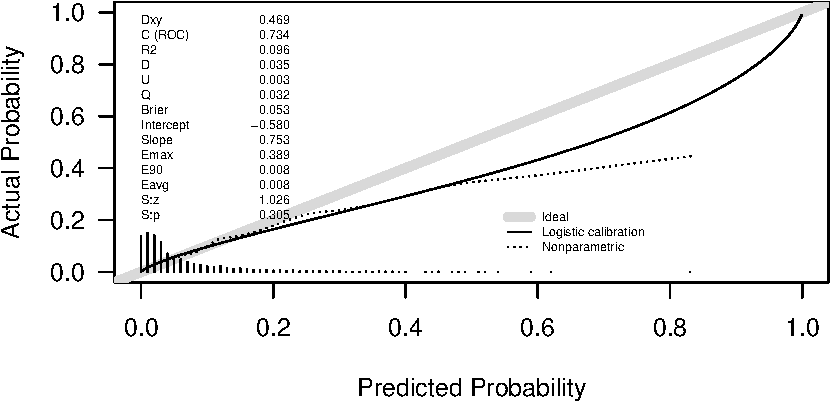
\includegraphics[width=1\linewidth]{greenwell-ebm_files/figure-latex/tic-ebm-calibration-1} 

}

\caption[Calibration curve and validation statistics based on the the test set]{Calibration curve and validation statistics based on the the test set.}\label{fig:tic-ebm-calibration}
\end{figure}
\begin{Soutput}
#>           Dxy       C (ROC)            R2             D      D:Chi-sq 
#>  4.687465e-01  7.343733e-01  9.569165e-02  3.511593e-02  1.414637e+02 
#>           D:p             U      U:Chi-sq           U:p             Q 
#>            NA  3.028332e-03  1.411333e+01  8.616484e-04  3.208759e-02 
#>         Brier     Intercept         Slope          Emax           E90 
#>  5.346921e-02 -5.796053e-01  7.534482e-01  3.888433e-01  7.959127e-03 
#>          Eavg           S:z           S:p 
#>  7.931846e-03  1.025679e+00  3.050429e-01
\end{Soutput}
\end{Schunk}

After training a model, it's often desirable to have a way to persist
the model for future use without having to retrain it. In R, we can
typically save the result of a model using \texttt{saveRDS()}.
Alternatively, some packages provide a more native solution, like
CRANpkg\{xgboost\}'s \texttt{xgb.save()} function. These solutions will
not work here since the connection to the underlying Python object is
lost once the session is finished. The proper way to handle this is to
use \pkg{reticulate}'s \texttt{py\_save\_object()} and
\texttt{py\_load\_object()} functions to save and load the underlying
Python object. This works by serializing the fitted EBM object using
Python's \pkg{pickle} module. Advanced \pkg{reticulate} users could also
rely on rely on the \pkg{joblib} module or even exporting the fitted
model to ONNX (Open Neural Network Exchange) via the \pkg{ebm2onnx}
module, depending on the need. For more details on persisiting a fitted
model in Python visit
\url{https://scikit-learn.org/stable/model_persistence.html}. Here we'll
show how to persist a fitted EBM model using both \pkg{pickle} (through
\pkg{reticulate}'s built-in functions mentioned above), as well as
\pkg{joblib}.

Note that a serialized \texttt{"EBM"} object get stripped of the
\texttt{"EBM"} class which is used for calling various methods, like
\texttt{plot()}, which we'll discuss later. To overcome that issues, we
provide an \texttt{as.ebm()} function for adding on the appropriate
class. This of course also means that you can import EBM models fitted
with the Python \pkg{interpret} module into R for use with
\texttt{print()}, \texttt{plot()}, etc.

\begin{Schunk}
\begin{Sinput}
# Save a fitted EBM model
reticulate::py_save_object(tic_ebm, filename = "tic_ebm.pkl")

# Load a pickled EBM model
(ebm_obj <- reticulate::py_load_object("tic_ebm.pkl"))
\end{Sinput}
\begin{Soutput}
#> ExplainableBoostingClassifier(early_stopping_tolerance=0,
#>                               interaction_smoothing_rounds=100,
#>                               learning_rate=0.04, max_leaves=2, min_hessian=0.0,
#>                               smoothing_rounds=500)
\end{Soutput}
\begin{Sinput}
(tic_ebm <- as.ebm(ebm_obj))  # adds "EBM" class for using print(), plot(), etc.
\end{Sinput}
\begin{Soutput}
#> 
#> Call:
#> NULL
#> 
#> Python object:
#> ExplainableBoostingClassifier(early_stopping_tolerance=0,
#>                               interaction_smoothing_rounds=100,
#>                               learning_rate=0.04, max_leaves=2, min_hessian=0.0,
#>                               smoothing_rounds=500)
#> 
#> Number of features: 85 
#> Number of terms: 162 
#> Number of interactions: 77 
#> Intercept: -3.364 
#> Objective: log_loss 
#> Link function: logit
\end{Soutput}
\end{Schunk}

Note that the original function call prints as \texttt{NULL} since it's
impossible to determine from the specific object we called
\texttt{as.ebm()} on.

In the specific case of an EBM, it may be more useful to use Python's
\pkg{joblib} module, which provides the \texttt{joblib.dump()} and
\texttt{joblib.load()} function for serializing and deserializing a
Python object, respectively; this approach is more efficient on objects
that carry large \pkg{numpy} arrays internally as is usually the case
for a fitted EBM model (all the term contributions, etc. are stored as
\pkg{numpy} arrays). As of this writing, \pkg{reticulate} does not
support \pkg{joblib} through any convenience function (e.g., like
\texttt{py\_save\_object()}), so we'll need to interface with the module
directly, as shown below:

\begin{Schunk}
\begin{Sinput}
joblib <- reticulate::import("joblib")  # assumes joblib module is available

# "Dump" the fitted EBM model into a pickle file
joblib$dump(tic_ebm, filename = "tic_ebm_joblib.pkl")
\end{Sinput}
\begin{Soutput}
#> [1] "tic_ebm_joblib.pkl"
\end{Soutput}
\begin{Sinput}
# Load a pickled EBM model
(tic_ebm <- as.ebm(joblib$load("tic_ebm_joblib.pkl")))
\end{Sinput}
\begin{Soutput}
#> 
#> Call:
#> NULL
#> 
#> Python object:
#> ExplainableBoostingClassifier(early_stopping_tolerance=0,
#>                               interaction_smoothing_rounds=100,
#>                               learning_rate=0.04, max_leaves=2, min_hessian=0.0,
#>                               smoothing_rounds=500)
#> 
#> Number of features: 85 
#> Number of terms: 162 
#> Number of interactions: 77 
#> Intercept: -3.364 
#> Objective: log_loss 
#> Link function: logit
\end{Soutput}
\end{Schunk}

Fitted \texttt{"EBM"} objects can be understood and visualized using the
generic \texttt{plot()} method. By default, \texttt{plot()} relies on
\CRANpkg{ggplot2} \citep{R-ggplot2} for variable importance and main
effect plots; for visualizing pairwise interactions, it relies on
\CRANpkg{lattice}'s \texttt{levelplot()} function. For convenience,
we'll also use \CRANpkg{patchwork} \citep{R-patchwork} for configuring
the layout for displays with multiple plots.

Below, we use the \texttt{plot()} method to display a few global
summaries of the fitted model. First, we display the overall term
importance scores. By default, all terms are plotted so it's a good idea
to set the \texttt{n\_features} argument to something reasonable if the
model contains lots of terms. Here we tell it to display the top 15
terms in the model. The importance scores are computed as the mean
absolute score from each term in the model.

\begin{Schunk}
\begin{Sinput}
library(ggplot2)
library(patchwork)

theme_set(theme_bw())  # my preferred theme for ggplot2

# Plot feature importance
plot(tic_ebm, n_terms = 15)  
\end{Sinput}
\begin{figure}[!htb]

{\centering 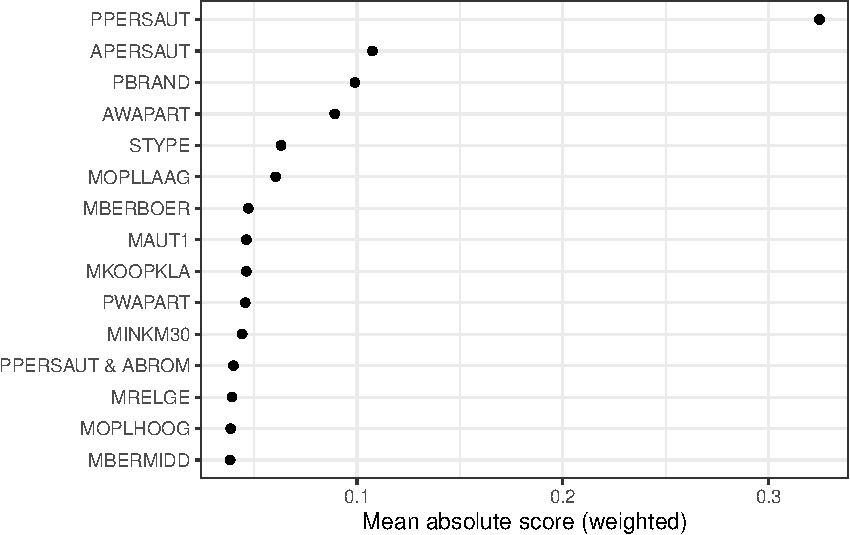
\includegraphics[width=1\linewidth]{greenwell-ebm_files/figure-latex/tic-ebm-importance-1} 

}

\caption[Term importance scores computed as the mean absolute score for each term in the fitted model]{Term importance scores computed as the mean absolute score for each term in the fitted model.}\label{fig:tic-ebm-importance}
\end{figure}
\end{Schunk}

The default behavior is to produce a dotchart, but you can switch to a
bar plot by setting \texttt{geom\ =\ "col"} in the call to
\texttt{plot()}. Setting \texttt{horizontal\ =\ TRUE} will also produce
a plot that's been flipped on its axes. See \texttt{?ebm::plot.EBM} for
details.

Next, we'll plot the main effect for \texttt{PPERSAUT}, the highest
rated term in the model, by setting \texttt{term\ =\ "PPERSAUT"} in the
call to \texttt{plot()}; note that this is just a plot of shape function
\(f\left(\mathtt{PPERSAUT}\right)\) from \eqref{eqn:ebm}. It's good
practice to include some information regarding the distribution of ther
variable of interest to help avoid extrapolation and over interpreting
such plots.

\begin{Schunk}
\begin{Sinput}
plot(tic_ebm, "PPERSAUT", horizontal = TRUE) +  # main effect plot
  ggplot(tictrn, aes(PPERSAUT)) +  # add distribution plot
  geom_bar() + 
  scale_x_discrete(drop = FALSE) +  # don't drop zero counts 
  xlab("") +
  coord_flip()
\end{Sinput}
\begin{figure}[!htb]

{\centering 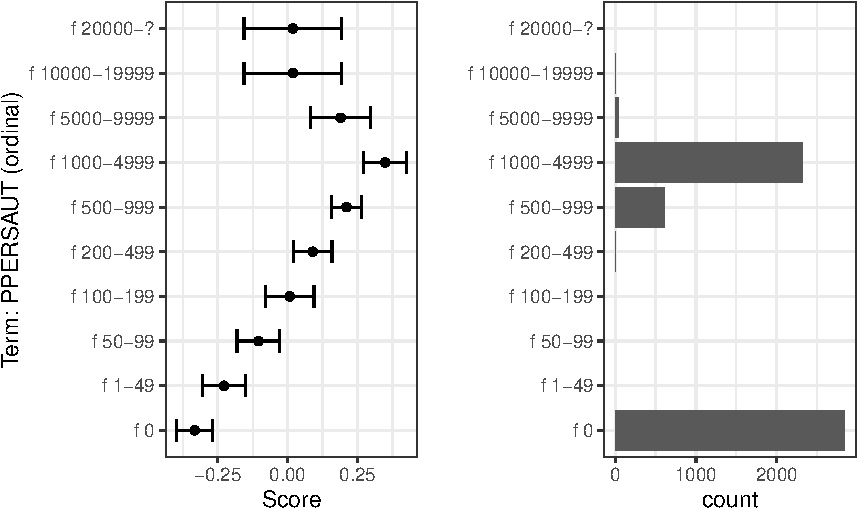
\includegraphics[width=1\linewidth]{greenwell-ebm_files/figure-latex/tic-ebm-term-PPERSAUT-1} 

}

\caption[Main effect of $\mathtt{PPERSAUT}$]{Main effect of $\mathtt{PPERSAUT}$.}\label{fig:tic-ebm-term-PPERSAUT}
\end{figure}
\end{Schunk}

\texttt{PPERSAUT} is an ordered factor representing the contribution
level for car policies. The left side of Figure
\ref{fig:tic-ebm-term-PPERSAUT} shows a generally increasing
relationship between contribution to car policies and the log odds of
buying a mobile home policy. The distribution of \texttt{PPERSAUT} in
the training data is also shown on the right side of Figure
\ref{fig:tic-ebm-term-PPERSAUT}. You can similarly display heatmaps for
pairwise interactions, but we'll reserve this for an example in a later
section of this paper.

One attractive feature of the \pkg{interpret} Python module is the use
of interactive graphics and dashboards (e.g., via Plotly
\citep{plotly}). This feature is not available in the corresponding R
package. Since we can expose the full functionality of the Python
version through \pkg{reticulate}, the \texttt{plot()} function can be
used to also produce the same interactive graphics. These can be viewed
either in the browser (the default) or in an interactive viewer like the
ones built into RStudio or VS Code. Below we reproduce the main effect
term for \texttt{PPERSAUT} using an interactive Plotly/HTML-based
graphic that will open by default in a browser. This will work for any
of the visualizations discussed in this paper. Note, however, that while
\pkg{ebm} supports multiclass outcomes, only interactive visualizations
are available (i.e., no static \pkg{ggplot2}-based plots). Of course,
these plots can always be constructed quite easily following the
approach discussed at the end of this section.

\begin{Schunk}
\begin{Sinput}
plot(tic_ebm, term = "PPERSAUT", interactive = TRUE)
\end{Sinput}
\end{Schunk}

\begin{Schunk}
\begin{figure}[!htb]

{\centering 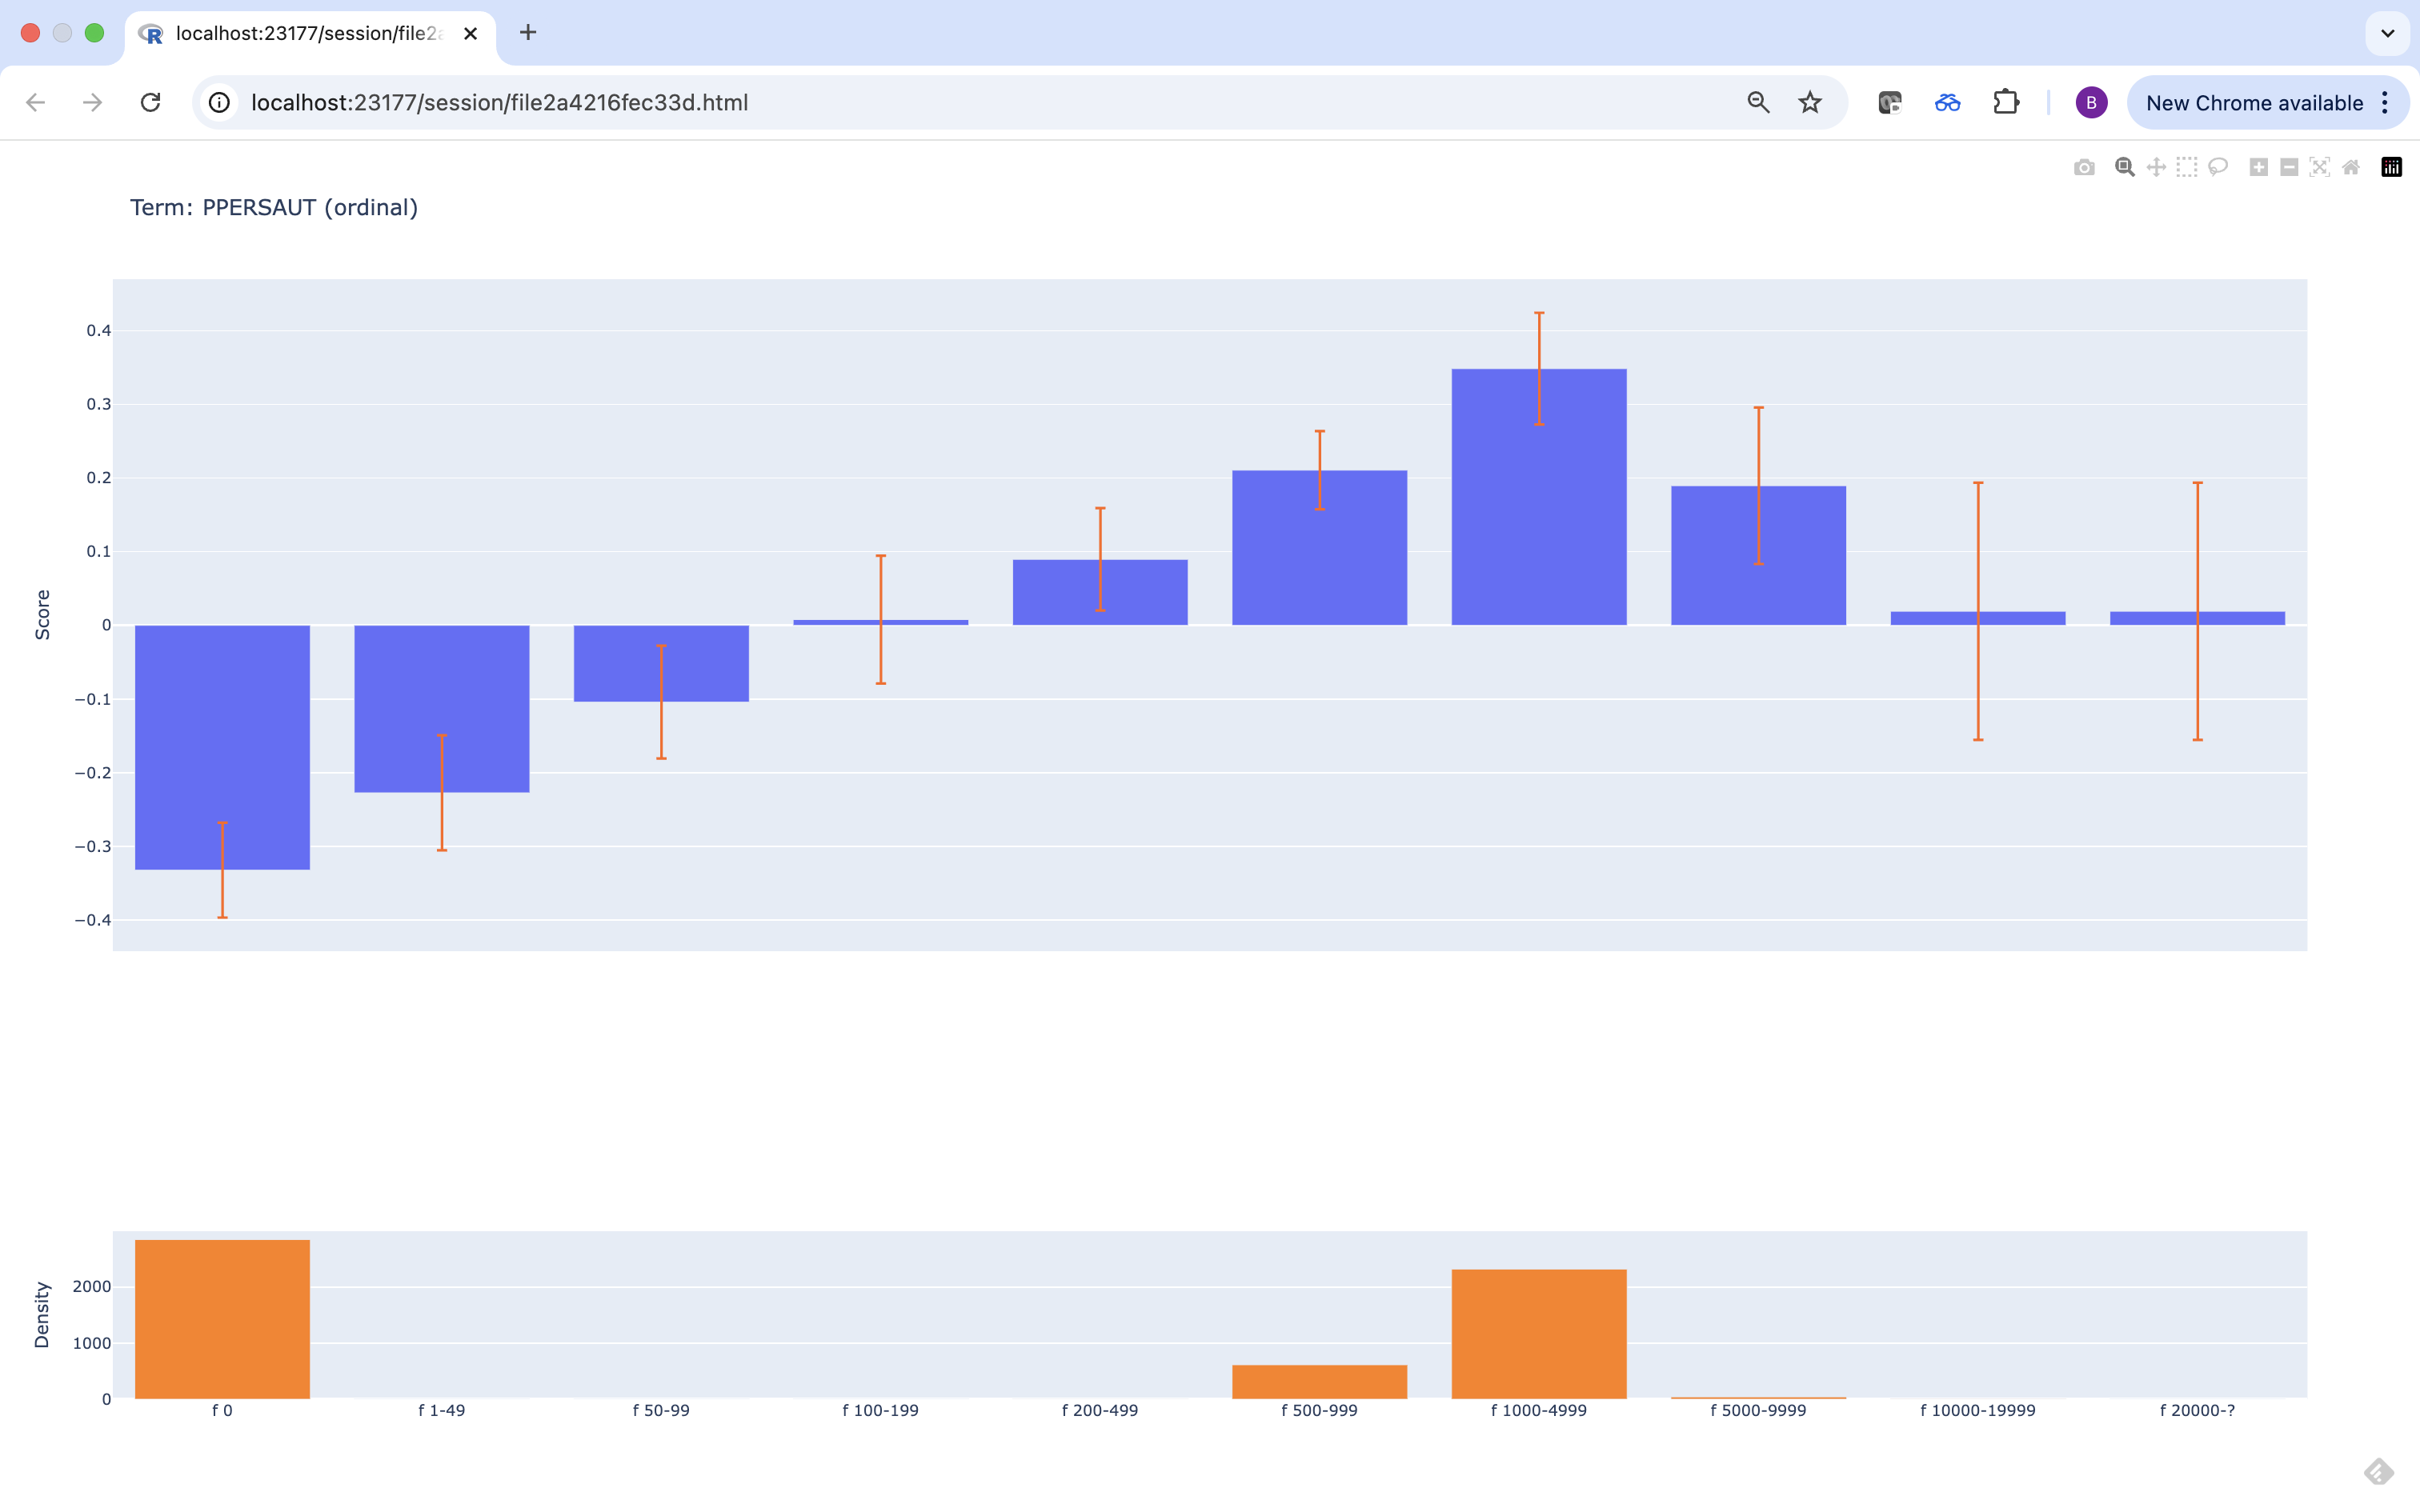
\includegraphics[width=1\linewidth]{images/screenshot} 

}

\caption[Screenshot of an interactive visualization for the main effect of $\mathtt{PPERSAUT}$ displayed in a Google Chrome browser]{Screenshot of an interactive visualization for the main effect of $\mathtt{PPERSAUT}$ displayed in a Google Chrome browser.}\label{fig:tic-ebm-term-PPERSAUT-html-hide}
\end{figure}
\end{Schunk}

Let's look at the second most important term, \texttt{APERSAUT}, which
corresponds to a continuous feature representing the number of car
policies owned. The main effect for \texttt{APERSAUT} is displayed in
the left side of Figure \ref{fig:tic-ebm-term-APERSAUT}. We might expect
there to be an increasing monotonic relationship between
\texttt{APERSAUT} and the log odds of buying a mobile home policy. In
fact, it's often desirable that the shape functions
\(f_j\left(x_j\right)\) in \eqref{eqn:ebm} be constrained in some way.
This may be due to business considerations, or because of some a priori
belief about the underlying relationships between the predictors and the
response. In such cases, we may wish to enforce a type of constraint
called monotonicity on some of the terms in the model. This means, for
example, that the relationship between \(x_j\) and \(y\), as modeled
through \(f_j\left(x_j\right)\) should always be increasing or
decreasing. For instance, a monotonic increasing relatiobnship would
ensure that \(f_j\left(x_j\right) \ge f_j\left(x_j'\right)\) whenever
\(x_j \ge x_j'\) (and vice versa for a decreasing monotonic
relationship).

To illustrate the idea, we'll enforce a decreasing monotonic
relationship between \texttt{APERSAUT} and the log odds of purchasing a
mobile policy (\texttt{CARAVAN}). While we can enforce monotonic
constraints via the \texttt{monotone\_constraints} argument in the call
to \texttt{ebm()}, the \pkg{interpret} authors generally recommend
forcing monotonicity by post-processing the graphs of the fitted model
instead using isotonic regression. This is the recommended approach as
it prevents the model from compensating for the monotonicity constraints
by learning non-monotonic effects in other highly-correlated features.
We can follow this route by calling the \texttt{\$monotonize()} method
that's bound to the fitted \texttt{"EBM"} object. Note that calling this
method will modify the original object in place, so to preserve the
original object, we'll also call the \texttt{\$copy()} bound method to
make a deep copy. Additionally, we lose any uncertainty associated with
the term from the outer bagging in the original model.

\begin{Schunk}
\begin{Sinput}
tic_ebm_mono <- as.ebm(tic_ebm$copy())  # make a deep copy to leave original intact
tic_ebm_mono$monotonize("APERSAUT", increasing = FALSE)
\end{Sinput}
\begin{Soutput}
#> ExplainableBoostingClassifier(early_stopping_tolerance=0,
#>                               interaction_smoothing_rounds=100,
#>                               learning_rate=0.04, max_leaves=2, min_hessian=0.0,
#>                               smoothing_rounds=500)
\end{Soutput}
\begin{Sinput}
# Display results side by side
plot(tic_ebm, term = "APERSAUT") + ggtitle("Original") +
  plot(tic_ebm_mono, term = "APERSAUT") + ggtitle("Monotonized")
\end{Sinput}
\begin{figure}[!htb]

{\centering 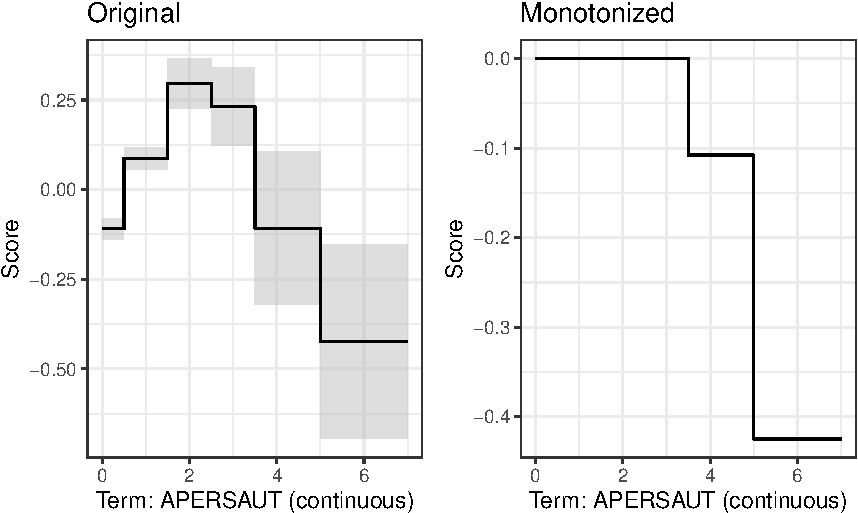
\includegraphics[width=1\linewidth]{greenwell-ebm_files/figure-latex/tic-ebm-term-APERSAUT-1} 

}

\caption[Main effect for $\mathtt{APERSAUT}$ Left]{Main effect for $\mathtt{APERSAUT}$ Left: Original (i.e., unconstrained) effect. Right: Decreasing monotonic effect through post-pocessing the left figure using isotonic regression.}\label{fig:tic-ebm-term-APERSAUT}
\end{figure}
\end{Schunk}

While the \pkg{ebm} package functions do not expose 100\% of the
functionality available in the corresponding Python module, this example
shows that you can pretty much do anything you need by interacting
directly with the underlying Python objects (the magic happens through
\pkg{reticulate}). For example, to reproduce the original HTML-based
visualization, which will be displayed in a browser, you can do the
following:

\begin{Schunk}
\begin{Sinput}
idx <- as.integer(which(tic_ebm$term_names_ == "APERSAUT") - 1L) 
plt <- tic_ebm$explain_global()$visualize(idx)
plt$show()  # should open in a browser; can also call `plt$write_html("<path/to/file.html>")`
\end{Sinput}
\end{Schunk}

Details aside, you can access the data to recreate the plot (like the
\texttt{plot()} method does), by coercing the internal Python plotly
object to an ordered dictionary which \pkg{reticulate} will
automatically convert to a list. For instance, the following snippet of
code extracts the main data used in generating the previous plot.

\begin{Schunk}
\begin{Sinput}
plt$to_ordered_dict()$data[[1L]]
\end{Sinput}
\begin{Soutput}
#> $line
#> $line$shape
#> [1] "hv"
#> 
#> $line$width
#> [1] 0
#> 
#> 
#> $marker
#> $marker$color
#> [1] "#444"
#> 
#> 
#> $mode
#> [1] "lines"
#> 
#> $name
#> [1] "Lower Bound"
#> 
#> $type
#> [1] "scatter"
#> 
#> $x
#> [1] 0.0 0.5 1.5 2.5 3.5 5.0 7.0
#> 
#> $xaxis
#> [1] "x"
#> 
#> $y
#> [1] -0.13932080  0.05711372  0.22630598  0.12305663 -0.32091075 -0.69571839
#> [7] -0.69571839
#> 
#> $yaxis
#> [1] "y"
\end{Soutput}
\end{Schunk}

The visualizations discussed so far are examples of \emph{global
explanations}. We can also explain the model's output at the local
(i.e., prediction) level. This is more commonly done for general machine
learning models using techniques like SHAP (SHapley Additive
exPlanations) \citep{lundberg-2017-shap} and LIME (Local Interpretable
Model-agnostic Explanations) \citep{ribeiro-2016-lime}. Techniques like
these typically make assumptions about independence and so forth and
only provide an approximation to how features contribute to a model's
output. With EBMs, we can visualize exactly how each term in the model
contributes to a specific prediction (this is true for GAMs in general).

Below, we call the \texttt{plot()} method to explain the prediction
associated with the first instance of the test sample. The EBM model
predicts a very low probability of purchasing a mobile home policy
(\(\hat{p}\left(\boldsymbol{x}\right) = 0.0316\)), and we'd like to know
how each term in the model contributed to that prediction. Note that we
need to specify a couple of additional arguments here. In particular, we
need to set \texttt{local\ =\ TRUE} and provide the input features as a
data frame via the \texttt{X} argument. You can optionally provide the
response values, but this only affects the interactive version (i.e.,
when setting \texttt{interactive\ =\ TRUE}) by displaying the associated
predicted and observed response value at the top. The results are
displayed in Figure \ref{fig:tic-ebm-local}.

\begin{Schunk}
\begin{Sinput}
newx <- subset(tictst[1L, ], select = -CARAVAN)
newy <- tictst$CARAVAN[1L]  # not useful unless `interactive = TRUE`
plot(tic_ebm, local = TRUE, X = newx, y = newy)
\end{Sinput}
\begin{figure}[!htb]

{\centering 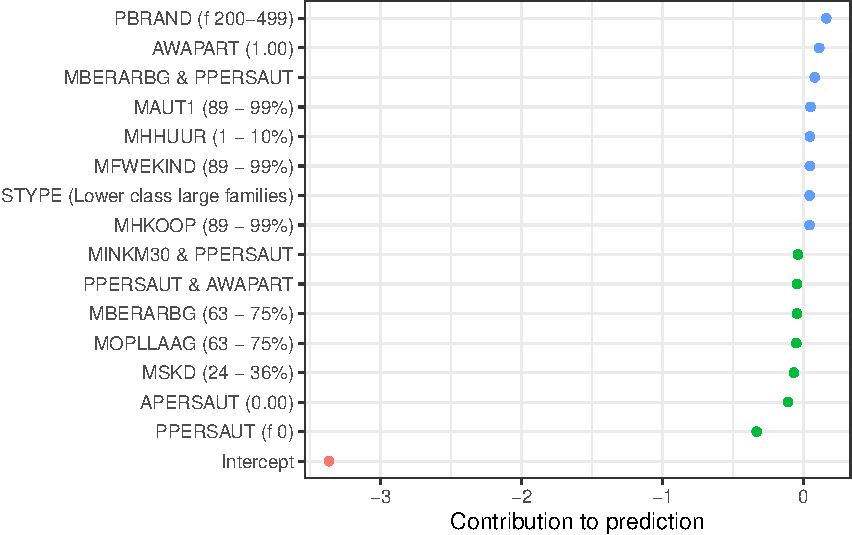
\includegraphics[width=1\linewidth]{greenwell-ebm_files/figure-latex/tic-ebm-local-1} 

}

\caption[ABC..]{ABC...}\label{fig:tic-ebm-local}
\end{figure}
\end{Schunk}

From Figure \ref{fig:tic-ebm-local} we can see that the biggest drivers
for a low score were the fact that this customer did not appear to have
or make any contribution toward existing car policies.

\subsection{Predicting ALS progression (the DREAM challenge prediction
prize)}\label{predicting-als-progression-the-dream-challenge-prediction-prize}

In this section, we'll look at a brief example using the ALS data from
Efron and Hastie (2016, 349). A description of the data, along with the
original source and download instructions, can be found at
\url{https://hastie.su.domains/CASI/data.html}.

These data concern 1822 observations on \emph{amyotrophic lateral
sclerosis} (ALS or Lou Gehrig's disease) patients. The goal is to
predict ALS progression over time, as measured by the slope (or
derivative) of a functional rating score (i.e., column \texttt{dFRS}),
using 369 available predictors obtained from patient visits. The data
were originally part of the DREAM-Phil Bowen ALS Predictions Prize4Life
challenge. The winning solution \citep{kuffner-2015-als} used a Bayesian
tree ensemble quite similar to a random forest, while
\cite[chap. 17]{efron-2016-casi} analyzed the data using gradient tree
boosting via the R package \CRANpkg{gbm} \citep{R-gbm}.

Below, we load in the ALS data from a URL and fit a default EBM. Note
that the data already contain an indicator for the train/test splits, so
we use that to split the data and discard the column after. We also
compute the MSE on the test set.

\begin{Schunk}
\begin{Sinput}
# Laod data and split into train/test sets
url <- "https://hastie.su.domains/CASI_files/DATA/ALS.txt"
als <- read.table(url, header = TRUE)
alstrn <- subset(als, subset = !testset, select = -testset)  # training data
alstst <- subset(als, subset = testset, select = -testset)   # test data

# Fit a default EBM regressor
(als_ebm <- ebm(dFRS ~ ., data = alstrn, objective = "rmse"))
\end{Sinput}
\begin{Soutput}
#> 
#> Call:
#> ebm(formula = dFRS ~ ., data = alstrn, objective = "rmse")
#> 
#> Python object:
#> ExplainableBoostingRegressor(early_stopping_tolerance=0)
#> 
#> Number of features: 369 
#> Number of terms: 702 
#> Number of interactions: 333 
#> Intercept: -0.6802 
#> Objective: rmse 
#> Link function: identity
\end{Soutput}
\begin{Sinput}
# Compute MSE on the test set
pred <- predict(als_ebm, newdata = alstst)
(mse_tst <- mean((alstst$dFRS - pred)^2))
\end{Sinput}
\begin{Soutput}
#> [1] 0.2669048
\end{Soutput}
\end{Schunk}

The fitted EBM model contains 702 terms (369 main effect terms, one for
each predictor, and 333 pairwise interaction terms) plus an intercept.
The mean square error for this model on the test data was 0.267. The top
10 terms are displayed in Figure \ref{fig:als-ebm-importance} below.
Here, we see that \texttt{Onset.Delta} is by far the most important
predictive feature in the model.

\begin{Schunk}
\begin{Sinput}
plot(als_ebm, n_terms = 10)  # Figure XYZ
\end{Sinput}
\begin{figure}[!htb]

{\centering 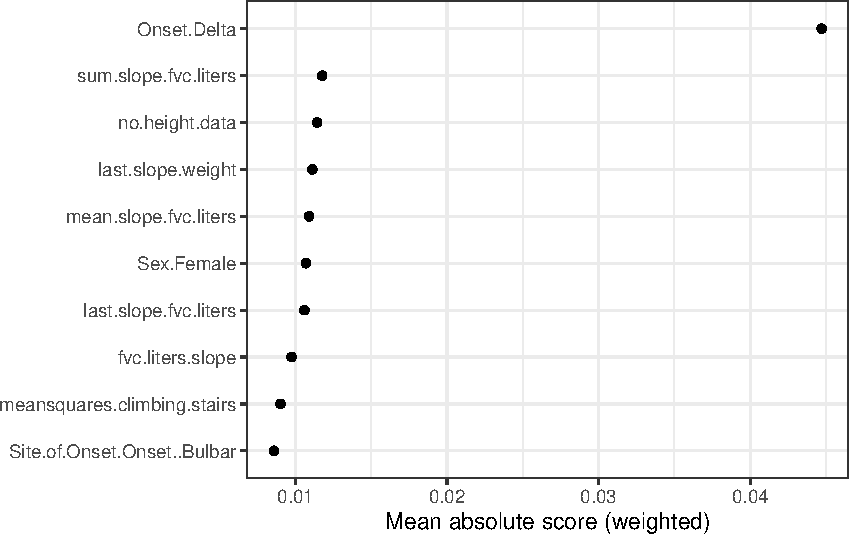
\includegraphics[width=1\linewidth]{greenwell-ebm_files/figure-latex/als-ebm-importance-1} 

}

\caption[ABC]{ABC.}\label{fig:als-ebm-importance}
\end{figure}
\end{Schunk}

As briefly mentioned in the previous example, we can also plot pairwise
interaction effects using a heatmap (or contour plot). Below we plot the
term contribution for
\(f\left(\mathtt{Onset.Delta}, \mathtt{last.slope.weight}\right)\).

\begin{Schunk}
\begin{Sinput}
plot(als_ebm, term = c("Onset.Delta", "last.slope.weight"))
\end{Sinput}
\begin{figure}[!htb]

{\centering 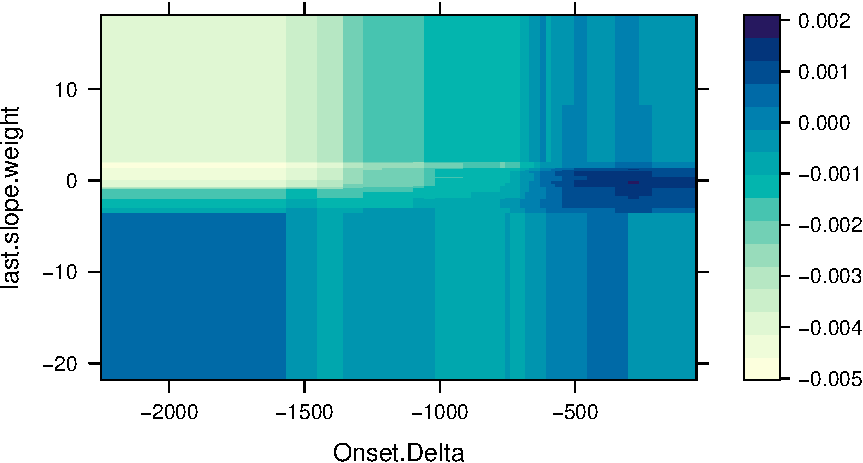
\includegraphics[width=1\linewidth]{greenwell-ebm_files/figure-latex/als-ebm-pairwise-interaction-1} 

}

\caption[ABC]{ABC.}\label{fig:als-ebm-pairwise-interaction}
\end{figure}
\end{Schunk}

Compared to ``black-box'' models, like random forests and deep neural
networks, EBMs are considered ``glass-box'' models that can be
competitively accurate while also maintaining a higher degree of
transparency and explainability. However, EBMs become readily less
transparent and harder to interpret in high-dimensional settings with
many predictor variables; they also become more difficult to use in
production due to increases in scoring time. We propose a simple
solution based on the least absolute shrinkage and selection operator
(LASSO) that can help introduce sparsity by reweighting the individual
model terms and removing the less relevant ones, thereby allowing these
models to maintain their transparency and relatively fast scoring times
in higher-dimensional settings. In short, post-processing a fitted EBM
with many (i.e., possibly hundreds or thousands) of terms using the
LASSO can help reduce the model's complexity and drastically improve
scoring time. For methodological (and software) details, see
\citet{greenwell-2023-explainable}.

We'll illustrate the basic idea using the previous model, which contains
703 total terms comprised of the main effects, pairwise interactions,
and an intercept.

In the next chunk, we'll construct data matrices consisting of the
individual term contributions for both the train and test sets. For
example, the \(j\)-th column of \texttt{X\_trn} is given by the
contribution of the \(j\)-th term of the model
\(\left\{f_j\left(x_{ij}\right)\right\}_{i=1}^n\) over the training set.
In particular, note that
\texttt{rowSum(terms\_trn)\ +\ fit\$intercept\_} is equivalent to
calling \texttt{predict(fit,\ newdata\ =\ X\_trn)}. These data matrices
will be used as input to the LASSO shortly after.

\begin{Schunk}
\begin{Sinput}
X_trn <- predict(als_ebm, newdata = alstrn, type = "terms")
X_tst <- predict(als_ebm, newdata = alstst, type = "terms")
colnames(X_trn) <- colnames(X_tst) <- als_ebm$term_names_
print(dim(X_trn))  # same rows as alstrn, but one column for each term in model
\end{Sinput}
\begin{Soutput}
#> [1] 1197  702
\end{Soutput}
\begin{Sinput}
# Sanity check (should be equivalent)
head(cbind(
  rowSums(X_trn) + c(als_ebm$intercept_),
  predict(als_ebm, newdata = alstrn)  # additive on link scale
))
\end{Sinput}
\begin{Soutput}
#>            [,1]       [,2]
#> [1,] -0.7866218 -0.7866218
#> [2,] -0.1947158 -0.1947158
#> [3,] -0.5743338 -0.5743338
#> [4,] -1.1612496 -1.1612496
#> [5,] -0.8793495 -0.8793495
#> [6,] -0.5021240 -0.5021240
\end{Soutput}
\end{Schunk}

Next, we use the
\href{https://cran.r-project.org/package=glmnet}{glmnet} package to fit
the LASSO path to the new data set comprised of the individual term
contributions. We then assess performance using the associated test set
and collect the results.

\begin{Schunk}
\begin{Sinput}
library(glmnet)

# Fit the LASSO regularization path using the term contributions as inputs
lasso <- glmnet(X_trn, y = alstrn$dFRS, lower.limits = 0, standardize = FALSE)

# Assess performance of fit using an independent test set
perf <- assess.glmnet(lasso, newx = X_tst, newy = alstst$dFRS)
perf <- do.call(cbind, args = perf)  # bind results into matrix

# Collect results and sort by number of non-zero coefficients/terms
res <- as.data.frame(cbind("n_terms" = lasso$df, perf, "lambda" = lasso$lambda))
head(res <- res[order(res$n_terms), ])
\end{Sinput}
\begin{Soutput}
#>    n_terms       mse       mae      lambda
#> s0       0 0.3203724 0.4583318 0.010792530
#> s1       1 0.3132038 0.4529917 0.009833751
#> s2       1 0.3072654 0.4484656 0.008960148
#> s3       1 0.3023472 0.4444106 0.008164153
#> s4       1 0.2982750 0.4410089 0.007438872
#> s5       1 0.2949041 0.4381329 0.006778023
\end{Soutput}
\end{Schunk}

Next, we'll compute the \texttt{lambda} value associated with the
smallest deviance (or half the log-loss). Here are the results for the
compressed EBM corresponding to this value of \texttt{lambda}:

\begin{Schunk}
\begin{Sinput}
lambda <- res[which.min(res$mse), "lambda"]
res[which.min(res$mse), ]
\end{Sinput}
\begin{Soutput}
#>     n_terms      mse       mae       lambda
#> s36      23 0.262219 0.4040236 0.0003789464
\end{Soutput}
\end{Schunk}

Finally, we can plot the results! On the left, we show the LASSO
coefficient path and on the right we show the test deviance as a
function of the number of terms in the compressed model.

\begin{Schunk}
\begin{Sinput}
par(mfrow = c(1, 2), mar = c(4, 4, 0.1, 0.1), cex.lab = 0.95, 
    cex.axis = 0.8, mgp = c(2, 0.7, 0), tcl = -0.3, las = 1)
plot(lasso, xvar = "lambda", col = adjustcolor("darkred", alpha.f = 0.3),
     xlab = "Log lambda")
abline(v = log(lambda), lty = 2, col = 1)
plot(res[, c("n_terms", "mse")], type = "l", las = 1,
     xlab = "Number of terms", ylab = "Test MSE")
abline(h = mse_tst, lty = 2, col = "darkred")
\end{Sinput}


\begin{center}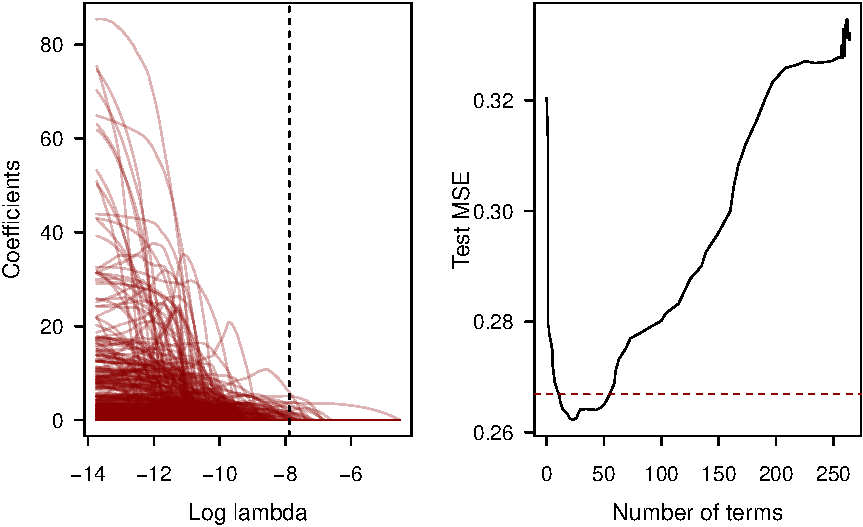
\includegraphics[width=1\linewidth]{greenwell-ebm_files/figure-latex/als-ebm-lassso-plot-1} \end{center}

\end{Schunk}

The test MSE for the compressed model is 0.262219\ldots{}

Lastly, we can call the \texttt{\$scale()} and \texttt{\$sweep()}
methods to reweight and purge any unused terms from the model:

\begin{Schunk}
\begin{Sinput}
als_ebm_lasso <- as.ebm(als_ebm$copy())
weights <- coef(lasso, s = lambda)  # LASSO coefficients (most are zero!)
weights <- setNames(as.numeric(weights), nm = rownames(weights))
for (i in seq_along(weights[-1L])) {
  idx <- as.integer(i - 1L)  # Sigh, Python indexing starts at 0
  als_ebm_lasso$scale(idx, factor = weights[i + 1])
}
als_ebm_lasso$intercept_ <- weights[1L]

# Remove unused terms!
als_ebm_lasso$sweep(terms = TRUE, bins = TRUE, features = FALSE)
\end{Sinput}
\begin{Soutput}
#> ExplainableBoostingRegressor(early_stopping_tolerance=0)
\end{Soutput}
\begin{Sinput}
length(als_ebm_lasso$term_names_)
\end{Sinput}
\begin{Soutput}
#> [1] 23
\end{Soutput}
\begin{Sinput}
plot(als_ebm_lasso)  # show new feature importance scores
\end{Sinput}


\begin{center}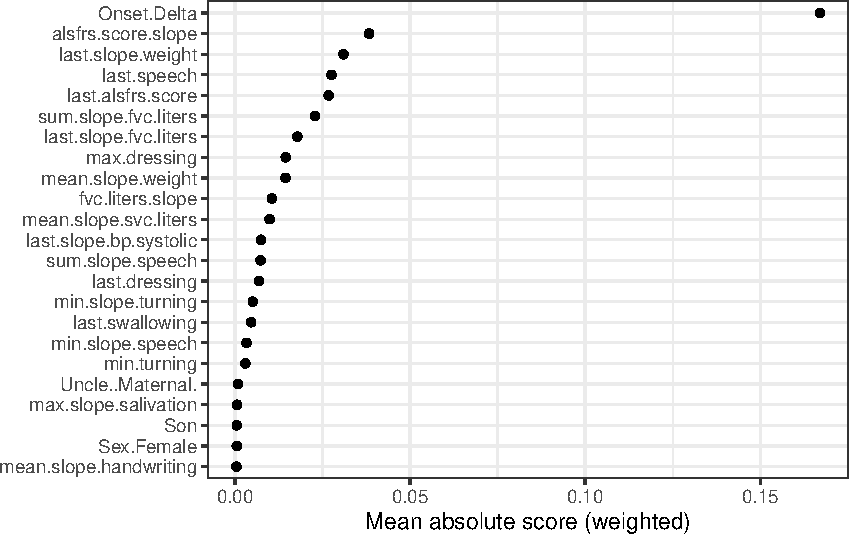
\includegraphics[width=1\linewidth]{greenwell-ebm_files/figure-latex/als-ebm-lasso-scale-1} \end{center}

\end{Schunk}

And just as a sanity check, we can see that the compressed (i.e.,
reduced) model does produce the right predictions. An ROC curve via the
\href{https://cran.r-project.org/package=pROC}{pROC} is also constructed
and shown below.

\begin{Schunk}
\begin{Sinput}
# Compare predictions between LASSO and compressed EBM (should be the same!)
head(cbind(
  "EBM (LASSO)" = predict(als_ebm_lasso, newdata = alstst),
  "LASSO" = predict(lasso, newx = X_tst, s = lambda, type = "response"))
)
\end{Sinput}
\begin{Soutput}
#>      EBM (LASSO)         s1
#> [1,]  -0.2869531 -0.2869531
#> [2,]  -0.3862899 -0.3862899
#> [3,]  -0.4750451 -0.4750451
#> [4,]  -0.2647092 -0.2647092
#> [5,]  -0.8570664 -0.8570664
#> [6,]  -1.0047789 -1.0047789
\end{Soutput}
\end{Schunk}

\citet{greenwell-2023-explainable} provide a similar compression
analysis applied to the CoIL 2000 example via interfacing directly with
the Python \pkg{interpret} module through \pkg{reticulate}.

\subsection{Parallelization}\label{parallelization}

TBD. Use bike share example here. Note that negative integers are
interpreted using \pkg{joblib}'s formula:
\texttt{n\_cpus\ +\ 1\ +\ n\_jobs}. For example, setting
\texttt{n\_jobs\ =\ -2} will result in using all threads except for one.
The default is \texttt{n\_jobs\ =\ -1} which results in using all
available CPUs.

TODO: Describe what's happening in the code. Also mention the defaults.
Below is a brief example using the \texttt{Bikeshare} data available in
\CRANpkg{ISLR2} \citep{R-ISLR2}. Outer bags are used to generate error
bounds and help with smoothing the graphs.

\begin{Schunk}
\begin{Sinput}
keep <- c("workingday", "temp", "weathersit", "mnth", "hr", "bikers") 
bikeshare <- ISLR2::Bikeshare[, keep]

# Use all CPUs (this is the default, which sets n_jobs = -1)
system.time({
  ebm1 <- ebm(bikers ~ ., data = bikeshare, objective = "poisson_deviance",
              inner_bags = 20, outer_bags = 16, n_jobs = -1)
})
\end{Sinput}
\begin{Soutput}
#>    user  system elapsed 
#>   0.052   0.009   7.487
\end{Soutput}
\begin{Sinput}
# Use one CPU
system.time({
  ebm2 <- ebm(bikers ~ ., data = bikeshare, objective = "poisson_deviance",
              inner_bags = 20, outer_bags = 16, n_jobs = 1)
})
\end{Sinput}
\begin{Soutput}
#>    user  system elapsed 
#>  46.094   0.547  46.809
\end{Soutput}
\begin{Sinput}
# Use all CPUs, but no bagging
system.time({
  ebm3 <- ebm(bikers ~ ., data = bikeshare, objective = "poisson_deviance",
              inner_bags = 0, outer_bags = 1, n_jobs = -1)
})
\end{Sinput}
\begin{Soutput}
#>    user  system elapsed 
#>   0.024   0.001   1.112
\end{Soutput}
\begin{Sinput}
# Plot results (Figure XYZ)
plot(ebm2, term = "temp") + plot(ebm3, term = "temp") 
\end{Sinput}
\begin{figure}[!htb]

{\centering 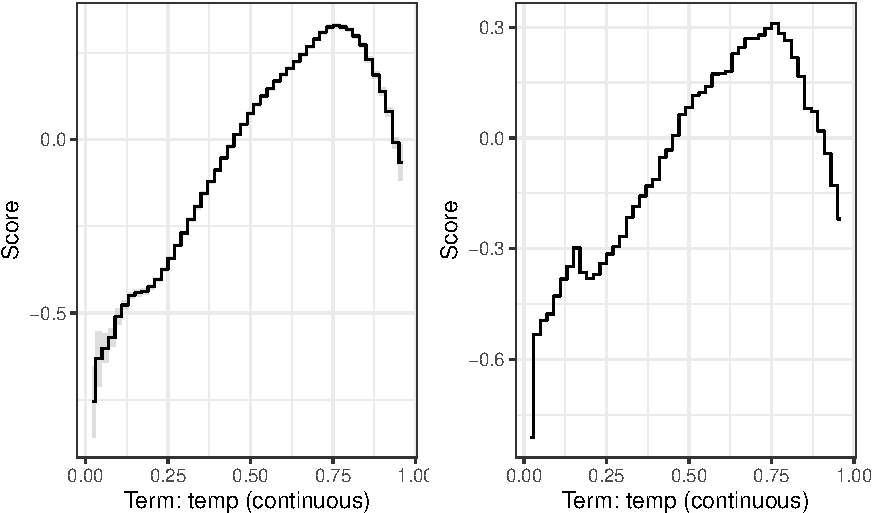
\includegraphics[width=1\linewidth]{greenwell-ebm_files/figure-latex/bikeshare-parallel-1} 

}

\caption[ABC]{ABC. Left: ABC. Right: ABC.}\label{fig:bikeshare-parallel}
\end{figure}
\end{Schunk}

\subsection{Tuning strategies}\label{tuning-strategies}

Recommended tuning strategies for EBMs are discussed in the
\pkg{interpret} module's FAQ: \url{https://interpret.ml/docs/faq.html}.
We outline the essential points here. Similar to random forests, the
default hyperparameters for EBMs tend to perform reasonably well on most
problems; hence, we stuck with the default for the examples in this
paper. A reasonable strategy is to train an initial model using the
defaults and looking through the learned functions to catch unexpected
or abnormal behavior---oftentimes, these graphs can help indicate which
parameters should be tuned. Here are some general recommendations from
the \pkg{interpret} module developers:

\begin{itemize}
\item
  For accuracy, it's generally recommend to set \texttt{outer\_bags} and
  \texttt{inner\_bags} to 25 or more each. This will significantly slow
  down the training time of the algorithm, and may be infeasible on
  larger data sets, but tends to produce smoother graphs with marginally
  higher accuracy. Note that the algorithm is parallelized at the outer
  bags level, so typically you'll pay a steeper price in terms of
  computing time for larger values of the inner bags parameter.
\item
  If you believe your model might be overfitting (e.g., large difference
  between train and test error, or high degrees of instability in the
  graphs), consider reducing \texttt{max\_bins} for smaller data sets
  (to clump more data together) and take a more aggressive approach to
  early stopping by decreasing \texttt{early\_stopping\_rounds} and
  increasing \texttt{early\_stopping\_tolerance}. Conversely, if you
  believe your model is underfitting, you can do the opposite of the
  previous suggestions (it might also be helpful to increase
  \texttt{max\_rounds}).
\item
  If several pairwise interaction effects seem realtively important
  (i.e., are appearing higher up on the term importance list/plot), then
  try increasing the maximum number of allowed interactions via the
  \texttt{interaction} argument.
\item
  For general tuning, it's recommended to sweep through
  \texttt{max\_bins} with values in the range 32--1024, and
  \texttt{max\_leaves} from 2--5. The potentialy improvements are
  typically marginal, but may help significantly on some data sets.
\end{itemize}

Detailed discussion on each hyperparameter available for tuning can be
found here: \url{https://interpret.ml/docs/hyperparameters.html}.

\section{Discussion}\label{discussion}

We gave a brief introduction to EBMs and a detailed walkthrough of the
new R interface provided by the \pkg{ebm} package.

\bibliography{greenwell-ebm.bib}

\address{%
Brandon M. Greenwell\\
University of Cincinnati\\%
Department of Operations, Business Analytics, and Information
Systems\\ Cincinnati, Ohio\\
%
\url{https://www.britannica.com/animal/quokka}\\%
\textit{ORCiD: \href{https://orcid.org/0000-0002-8120-0084}{0000-0002-8120-0084}}\\%
\href{mailto:greenwb@ucmail.uc.edu}{\nolinkurl{greenwb@ucmail.uc.edu}}%
}
